\documentclass[journal=jpccck,manuscript=article]{achemso}

\usepackage[version=3]{mhchem} 	% Formula subscripts using \ce{}
\usepackage{graphicx}
\graphicspath{{figure/}}		%FOLDER PATH for FIGURE
\usepackage[T1]{fontenc} 		% Use modern font encodings
\usepackage{siunitx}
\usepackage{chemformula}
\DeclareSIUnit\Molar{\textsc{m}}
% !TeX root = ./efcs.tex
\usepackage{xr} 
\externaldocument{Sup_info}
%======================New command========================
\newcommand{\uW}{\ensuremath{\,\mu\textrm{W}}}
\newcommand{\nm}{\ensuremath{\,\textrm{nm}}}
\newcommand{\um}{\ensuremath{\,\mu\textrm{m}}}
\newcommand{\mm}{\ensuremath{\,\textrm{mm}}}
\newcommand{\uM}{\ensuremath{\,\mu\textrm{M}}}
\newcommand{\mM}{\ensuremath{\,\textrm{mM}}}
\newcommand{\nM}{\ensuremath{\,\textrm{nM}}}
\newcommand{\pM}{\ensuremath{\,\textrm{pM}}}
\newcommand{\ns}{\ensuremath{\,\textrm{ns}}}
\newcommand{\us}{\ensuremath{\,\mu\textrm{s}}}
\newcommand{\ms}{\ensuremath{\,\textrm{ms}}}
\newcommand{\degree}{\ensuremath{\,^o\textrm{C}}}
%======================Author information====================== 
\author{Biswajit Pradhan}
\author{Saumyakanti Khatua}
\altaffiliation{Department of Chemistry, IIT-Gandhinagar, Ahmedabad - 382424, India}
\author{Ankur Gupta}
\altaffiliation{Department of Chemistry, IISER Bhopal, 462066, Madhya Pradesh, India}

\author{Thijs Aartsma}
\author{Gerard Canters}
\author{Michel Orrit}
\affiliation[Leiden University]
{Huygens-Kamerlingh Onnes Laboratory, Leiden University, 2300 RA Leiden, Netherlands}
\email{orrit@physics.leidenuniv.nl}
\phone{+31 (0)71 527 1720}
\title[]
{Gold-Nanorod-Enhanced FCS of Fluorophores with High Quantum Yield in Lipid Bilayers}

\abbreviations{FCS}
\keywords{American Chemical Society, \LaTeX}
%%%%%%%%%%%%%%%%%%%%%%%%%%%%%%%%%%%%%%%%%%%%%%%%%%%%%%%%%%%%%%%%%%
%%%%%%% Start the main part of the manuscript here.%%%%%%%%%%%%%%
%%%%%%%%%%%%%%%%%%%%%%%%%%%%%%%%%%%%%%%%%%%%%%%%%%%%%%%%%%%%%%%%%%
\begin{document}

%===========toc==========
\begin{tocentry}
\centering
\includegraphics[]{toc.png}
\end{tocentry}
%==========abstract==========
\begin{abstract}
	Plasmonic fluorescence enhancement is used to study fluorescence correlation spectroscopy (FCS) at higher concentrations than in regular diffraction-limited FCS experiments. Previous studies suffered from sticking to the substrate and were performed mainly with poorly emitting dyes. A lipid bilayer forms a passivating surface preventing sticking of the dye or the protein and allows for specific anchoring of probe molecules. For dyes with high quantum yields, the fluorescence background of unenhanced molecules is high, and the fluorescence enhancement is weak, less than about 10. Nonetheless, we show that FCS is possible at micromolar concentrations of the probe molecule. Enhanced FCS is recorded by selecting signals on the basis of their shortened lifetime. This selection enhances the contrast of the correlation by more than an order of magnitude. The lipid bilayer can be used to anchor biomolecules and perform enhanced FCS, as we show for a dye-labeled protein.
\end{abstract}
\pagebreak
%============================Introduction=====================================
\section{Introduction}
Fluorescence-based single-molecule detection helps exploring the structure and dynamics of complex biological matter.\cite{moerner1999illuminating,weiss1999fluorescence} Single-molecule signals can reveal a transient state during a chemical reaction, or report on the kinetics of processes as a function of position. Broadly there are two ways of studying single molecules: i) by immobilizing the molecule on a backgroundfree matrix or surface, ii) by dissolving the molecules in a fluid and measuring the signal fluctuation by fluorescence correlation spectroscopy (FCS).\cite{Magde1972} Both techniques require the molecule to possess a high quantum yield and good photostability. FCS studies are limited to concentrations in the pico- to nano-molar range, in view of the diffraction-limited detection volume of a few femtoliters (fL). As many biological reactions occur in the micromolar range\cite{craighead2006future}, smaller detection volumes are desirable to study these reactions by FCS.\\

Plasmonic nanostructures can both enhance molecular fluorescence in volumes smaller than the diffraction-limited volume and reduce the background fluorescence of the other molecules in the diffraction-limited volume. Zero-mode waveguides and antennas-in-box, in particular, both enhance fluorescence and reduce background.\cite{levene2003zeromode,kinkhabwala2012fluorescence,punj2013a,yuan2013thousandfold,punj2013gold} The effective fluorescence enhancement depends sensitively on the position and orientation of the molecule with respect to the nanoparticle. It originates from two factors, excitation enhancement and radiative enhancement. By confining the optical field into so-called hot spots with volumes much smaller than the diffraction limit,\cite{schuller2010plasmonics} plasmonic nanostructures enhance the incident field by up to a few orders of magnitude, leading to excitation enhancement.\cite{yuan2013thousandfold,anger2006enhancement,kinkhabwala2009large,acuna2012fluorescence,busson2012accelerated,holzmeister2014quantum,khatua2014resonant} They also alter the radiative and non-radiative decay rates of molecules in their vicinity. The ensuing radiative enhancement results from improved emission by the nanoantenna dipole induced by the molecular dipole. In addition, energy may be transferred from the molecule to the antenna resulting in non-radiative losses and energy dissipation in the metal. Changes in the radiative or non-radiative decay paths lead to altered, generally shortened fluorescence lifetimes.\cite{khatua2014resonant,liu2007quantized,lakowicz2001radiative,dulkeith2005gold,seelig2007nanoparticleinduced,muskens2007strong,pelton2015modified} Distance-dependent lifetime measurements show lifetime shortening up to 40 nm away from the metal surface.\cite{seelig2007nanoparticleinduced}\\

Noble-metal plasmonic nanostructures can be fabricated either by lithography or by colloid chemistry.\cite{zijlstra2011single} Whereas lithography can produce nanostructures with arbitrary geometries suitable for high optical confinement, it presents the disadvantages of complex processing, polycrystallinity, surface roughness, and high cost. Colloidal chemistry produces large numbers of highly crystalline nanostructures in a few basic shapes (spheres, rods, bipyramids, etc.) that are controllable to some extent, at a low cost. Among the basic nanoparticle shapes, nanorods\cite{yuan2013thousandfold} can be just as efficient as lithographically-made structures\cite{punj2013a,kinkhabwala2009large} in enhancing fluorescence. Gold nanorods confine the optical field more weakly than lithographically made gap structures, but they have the advantage of a narrow surface plasmon resonance, which can be tuned in the red and near infrared range by changing the rod’s aspect ratio.\cite{khatua2014resonant} The largest enhancement is achieved for a maximum overlap of the molecule’s excitation and fluorescence spectra, of the nanorod’s surface plasmon resonance, and of the excitation wavelength. Further advantages of gold nanoparticles are that they provide easy access of hot spots to diffusing molecules and that they can be inserted into complex environments such as living cells.\\

Confinement of light in volumes much smaller than the diffraction-limited volume combined with fluorescence enhancement open applications of FCS at micromolar dye concentrations. The correlation contrast in FCS decays as the square of the background intensity. To reduce background, most enhanced FCS experiments have been done on dyes with low quantum yields.\cite{kinkhabwala2012fluorescence,estrada200810000} Alternatively, a fluorescence quencher may be added to a dye with a high quantum yield (QY) to reduce background.\cite{punj2013a,punj2013gold} A metal box or cladding\cite{ghenuche2015matching} can also be fabricated around the nano structure to improve the correlation contrast against the background of unenhanced molecules. Both solutions have disadvantages, as a millimolar quencher concentration may be harmful to a living cell. Metal claddings are difficult to fabricate and to manipulate in a complex environment. Generalizing enhanced FCS to high-QY dyes would obviate these two problems and open plasmonic enhancement to biological marker dyes, most of which have high QY. Plasmonic enhancement may also help overcome other background sources such as autofluorescence in live-cell experiments. Indeed, as we show herein, even weak fluorescence enhancements suffice to overcome background in FCS experiments. Moreover, fluorescence photons with short emission times may be selected as was done by Acuna et al\cite{acuna2012fluorescence} further to improve the signal to noise ratio of enhanced FCS.\\

A further limitation in working with metal nanostructures on a solid substrate is the nonspecific interaction of the molecules with metal and substrate, which not only may affect the molecules’ functionality but also make measurements troublesome.\cite{kinkhabwala2012fluorescence,yuan2013thousandfold,zhang2009gold} Micellar solutions have been used to minimize sticking but are not ideal when studying biomolecules or performing experiments in live cells. We therefore need to suppress or mitigate nonspecific interactions of the dyes or biomolecules under study with the solid substrates supporting the structures. Living organisms use a lipid bilayer on their outer surface to prevent nonspecific interaction and protein fouling while allowing specific binding of membrane proteins.\cite{zhang2009gold,cooper2000cell} We have used a supported lipid bilayer to passivate the substrate.\cite{persson2012lipidbased,ller2012single,lohmuller2011supported} Supported bilayer can be self-assembled on solid surfaces (glass, silica, and similar polar surfaces) such that it forms a single, continuous membrane which possesses a high degree of lateral mobility by maintaining a very thin layer of water (1~nm) between substrate and bilayer.\cite{sackmann1996supported,CASTELLANA2006429,cremer1999formation,richter2006formation} Bilayers are also model systems to study diffusion in biological membranes. In standard experiments, diffusion in bilayers is studied on length scales limited by far-field resolution. Plasmonic enhancement gives us access to diffusion on the length scales of the near field, typically some tens of nm. Enhanced fluorescence experiments provide access to nanoscale diffusion in the vicinity of a gold nanorod.\\

Here we study fluorescence enhancement of a high-QY dye by immobilized single gold nanorods. Sticking of the dye to the glass substrate was prevented by coating the glass with a supported lipid bilayer formed from a zwitterionic lipid. We have characterized the properties of the enhanced signal and shown that its fluorescence decay is much faster than the far-field signal’s. Based on these time decay characteristics, we have filtered the near-field signal from the background of unenhanced dye fluorescence, thereby obtaining an improved FCS contrast. The same measurement provides both far-field and near-field diffusion components, and allows us to compare the diffusion kinetics in both regimes. We show that biomolecules can be successfully anchored in the bilayer, and that enhanced FCS can be performed while sticking and interaction with gold nanorods are prevented.\\
\begin{figure}
	\centering
	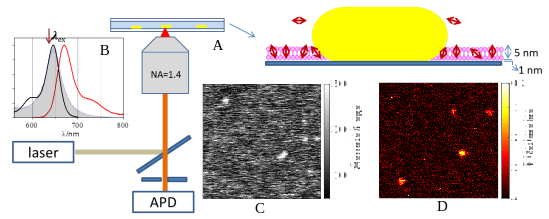
\includegraphics[width=\textwidth]{schematic.png}
	\caption{(A) Schematic diagram of the optical setup with a supported lipid bilayer (pink), ATTO 647N molecules (red) and a gold nanorod (yellow). (B) Absorption spectrum of ATTO 647N (black), fluorescence spectrum of ATTO 647N (red) and photoluminescence spectrum of a single gold nanorod (shaded area). Notice the overlap of the nanorod's SPR with the dye's absorption and emission spectra. (C) fluorescence intensity image (size $8~\uW \times 8~\uW$) and (D) fluorescence lifetime image (FLIM) of the same area of lipid bilayer. Note the lack of correlation between the fluorescent spots indicating dye aggregates in (C) and the short-lifetime spots in (D) indicating the rods.}
	\label{fig:schematic}
\end{figure}
%===========================Methods================================
\section{Methods}
\subsection{Gold nanorod immobilization}
Gold nanorods (AuNRs) were synthesized in cetyl trimethyl ammonium bromide (CTAB) using the seed-mediated growth method.\cite{nikoobakht2003preparation} The average dimension of the nanorods was $90~\nm\times50~\nm$. Fig. S\ref{SIfig: AuNR_uv-vis}B shows a scanning electron microscopy image of the nanoparticles. The bulk absorption spectra of these nanorods in Fig.S\ref{SIfig: AuNR_uv-vis}A show the longitudinal surface plasmon resonance (LSPR) at 640~\nm. The nanorod sample was diluted and the CTAB was washed away by centrifugation and re-suspension in milliQ water before use. Glass coverslips (Menzel-Glaser, $22~\mm\times 40\mm$, no. 1 thickness) were used for immobilization. The coverslips were sonicated in water (15~min) and acetone (15~min). Then they were rinsed in milliQ water several times and incubated in a $H_2O/NH_4OH/H_2O_2$ (5:1:1) bath at 70 \degree. The coverslips were rinsed several times with water and ethanol, and finally stored in ethanol. Before use the coverslips were flamed, and then ozone-cleaned for 15 minutes. The nanorods were spin-coated onto these coverslips at 2,000 rpm for 1 minute. These parameters gave us around 5 particles per $100~\um^2$ area and more than 90\% of them were single. The coverslips with the gold nanorods were then rinsed with water to remove remaining traces of CTAB, dried, and again ozone-cleaned for 30 minutes. This resulted in a very  hydrophilic surface. The coverslip was mounted in a homemade flow cell, where the surface was further prepared for confocal experiments.
\subsection{Supported lipid bilayer preparation}
Supported lipid bilayers were prepared from a zwitterionic lipid. Stock ampoules (25~mg) of 1-palmitoyl-2-oleoyl-sn-glycero-3-phosphocholine (POPC, see Fig.Sref{SIfig:chemical}B) were purchased from Avanti polar and stored at $-200$\degree immediately after receipt. The lipid powders were dissolved in chloroform and dried with argon in glass vials $1$~mg each and again stored at $-200$\degree until required. $4$~mL of Phosphate Buffered Saline (PBS) were added to the glass vial and the POPC was incubated for 1 hour at $40~$\degree (which gives a concentration of $0.25~$mg/mL). Then the vial was placed in the middle of a sonicator where the cavitation is greatest. It was sonicated for 30 minutes to produce small unilamellar vesicles (SUVs). The coverslips in the flow cell were hydrated by flowing PBS into the cell for 5 minutes. Then the coverslip was incubated with the SUV sample for 1 hour and washed with PBS to remove all free vesicles and debris. The vesicles rupture, spread and form a bilayer.\cite{richter2006formation} For protein anchoring, the vesicles for the bilayer were prepared from a mixture of POPC and DSPE-PEG(2000) Biotin (See Fig.S\ref{SIfig:chemical}C) with a ratio of 100:1.
\subsection{Labeling of the bilayer}
ATTO 647N NHS-ester (see Fig. S\ref{SIfig:chemical} for the structure) was purchased from ATTO-TEC. Before labeling, the reactive part of the dye (NHS-ester) was neutralized by incubating in 20~\mM Tris buffer pH 9 (the amine group present in Tris reacts with the ester). The dye in Tris pH 9 buffer at the concentration required by the experiment (vide infra) was passed into the flow cell. The dye goes into the bilayer only at higher pH probably because of the neutralization of charge on the nitrogen atom present on the head group of the lipid molecules. The dye mentioned in the whole discussion is ATTO 647N unless otherwise stated.
\subsection{Protein to bilayer anchoring}
Wild type (wt) azurin was prepared, purified and labeled as previously described.\cite{VANDEKAMP1990283,nicolardi2012top-down} ATTO 655 NHS ester was incubated with the azurin and azurin labeled at Lys122 was isolated and purified by chromatography on a MONO Q anion exchange column. Biotin-PEG-NHS (MW 3400, LaysanBio) was reacted with other lysine groups in the protein and the unreacted linkers were removed by centrifugal filtration. This labeled protein was then used for binding to the bilayer. A glass slide with a bilayer containing DSPE-PEG Biotin was incubated in a flow cell with neutravidin for 30 minutes and then washed with fresh PBS buffer. A 5~\nM solution of the labeled protein was flushed into the flow cell and left for 15 minutes and then the cell was washed again to remove the unbound proteins.
\subsection{Optical setup}
Measurements were carried out in a home-built confocal microscope. A $639~$\nm pulsed laser was controlled by PDL 800-B (PicoQuant) at 20 MHz repetition rate. This laser was used to excite the dye. A $532~$\nm Nd:YAG laser was used to measure the spectra of the gold nanorods. The $639~$\nm beam was passed through a narrow-band clean-up filter (LD01-640/8-25, Semrock) and coupled into a single-mode fiber (OZ optics). After passing the fiber the beam was collimated and passed through a quarter-wave plate to evenly excite nanorods irrespective of their orientation on the flat glass surface. The beam was reflected by a dichroic mirror (ZT640RDC, Chroma for $639~$\nm and T556lpxr-UF1 for $532~$\nm) and entered an oil immersion objective with numerical aperture (NA) of 1.4 (100X-oil, Zeiss) which focused it to a diffractionlimited spot of $265$\nm beam waist. The flow cell with the coverslip was mounted on a scanning stage controlled by nano-positioning piezo elements (P517.3CD, Physik Instrumente). The formation of the bilayer and its labeling were performed on this scanning stage and measurements were performed in each step. The epifluorescence was collected by the same objective and was separated from the excitation laser through an emission filter (ET655LP, Chroma for $639~$\nm laser) or notch filter (NF01-532U-25, Semrock for $532~$\nm laser). The emission was then spatially filtered by a $75~$\um pinhole and focused on a single-photon-counting module (SPCM-AQR-14, Perkin Elmer). The data were recorded through a photon counting PC-board (TimeHarp 200, PicoQuant) in time-tagged-time-resolved mode. The data acquisition and analysis were performed by using SymPhoTime (PicoQuant) software.
\subsection{Image and time trace recording}
The mounted sample was brought into focus and a typical area of $100~\um^2$ was imaged. The laser was parked on a gold nanorod and luminescence spectra were measured with a spectrograph equipped with a nitrogen-cooled CCD camera (Princeton Instruments SPEC-10). We made sure that the nanorods are single by verifying that the line shape of the luminescence spectrum was Lorentzian (Fig. \ref{fig:schematic}b, shaded area). A tris-neutralized solution of $50~$\pM and $100~$\nM ATTO 647N in Tris pH 9 was introduced into the flow cell. The sample was imaged in both XZ and XY planes. The luminescence intensity of the gold nanorods was not high enough to be distinguishable from the background. As the lifetime of the gold nanorod luminescence is much shorter than that of ATTO 647N (vide infra), fluorescence lifetime imaging (FLIM) was used to spot the nanorods (Fig. \ref{fig:schematic}D). Time traces were recorded in time-tagged-time-resolved mode at a power of $0.5~$\uW for burst analysis and $0.1~$\uW for FCS and were further analyzed with Symphotime software. To compare far-field and near-field, the laser was parked either on a gold nanorod or on the bilayer-covered glass surface.
%=========================RESULTS and DISCUSSION===============================
\section{Results and discussion}
To estimate the enhancement factor of single molecules, we flushed a $50~$\pM solution of ATTO 647N into the flow cell and allowed the dye to partition between solution and lipid bilayer, where diffusion is much slower. At this concentration we have less than $0.04$ molecules in our diffraction-limited volume of $0.5~$fL, making sure that the probability of observing more than one molecule in the far field at any time is very low. Figure \ref{fig:timetrace_hist}A shows a time trace of the gold nanorod in the absence of the dye. The intensity of the gold nanorod luminescence is around $50~$kcps. ATTO 647N in the bilayer far away from nanorod shows peaks with an intensity of around $100~$kcps as shown in Fig \ref{fig:timetrace_hist}C. The time trace and count histogram of ATTO 647N in the bilayer around a nanorod shows higher intensity bursts with a maximum intensity of around $460~$kcps. By subtracting the nanorod luminescence intensity, we get a maximum of $410~$kcps (Fig. \ref{fig:timetrace_hist}E) intensity which gives us a factor of four enhancement in the fluorescence. Histograms of photon counts per time bin of $100~$\us are presented for each time trace in Fig.\ref{fig:timetrace_hist}B, D, F. They show a much more intense tail of bright events for the enhanced trace in the presence of the rod, as observed previously.\cite{khatua2014resonant} Figure \ref{fig:enhnc_trajectories} presents four examples of time traces zoomed in around fluorescence bursts (Fig. \ref{fig:enhnc_trajectories}C) together with schemes qualitatively explaining the observed traces. Several combinations of far-field and near-field trajectories were observed. Fig \ref{fig:enhnc_trajectories}a (blue trace a) shows a molecule passing through the far-field without crossing the near field, the most probable event. Once in a while, a molecule passes from the far field to the near field (red b and magenta d) resulting in enhanced fluorescence. This is consistent with the enhancing hot spot being surrounded by the far-field spot. In a few rare cases, a molecule starts directly from the near-field (green c) and diffuses away through the far field. We attribute this sudden appearance to adsorption of a molecule from the solution (where it diffuses too fast to be visible) to the bilayer in the near-field area. Indeed, the dye being partly soluble in water and in the bilayer, it partitions in a dynamical equilibrium between the two phases. More examples of such bursts, including near-field traces suddenly interrupted by desorption or bleaching are described and briefly discussed in the Supporting Information (Section 4).\\
\begin{figure}
	\centering
	\includegraphics[]{timetrace_hist.png}
	\caption{Enhanced Fluorescence by a gold nanorod in a bilayer. Fluorescence time traces with binning time 100 μs. (A) Time trace of a gold nanorod in the absence of the dye, (C) Time trace with 50 pM ATTO 647N in the bilayer (E) Time trace with 50 pM ATTO 647N in the bilayer in presence of the gold nanorod. The corresponding histograms of counts are shown to the right of each time trace (B, D, F).}
	\label{fig:timetrace_hist}
\end{figure}
The four-fold enhancement found above for a high-QY dye in the bilayer is much lower than the enhancements observed earlier for poorly emitting dyes.\cite{yuan2013thousandfold} We ascribe this lower enhancement to reductions of both excitation and emission enhancements in our present case. We first consider the position of the dye molecules with respect to the rod’s tips. Because the dyes in the bilayer are confined in a $5~$\nm thick layer that is assumed to stick onto the glass substrate, they are largely outside the near-field hot spots at the tip of the $50~$\nm wide nanorod (see sketch in Fig.\ref{fig:schematic}), and are thus unable to explore the region of the hot spot with the highest intensity, resulting in a lower excitation enhancement than with 3D diffusion. Indeed, we observed a much higher enhancement of ATTO 647N when the molecules were allowed to explore the whole space in 3D solution around the gold nanorod (see Supporting Fig.S\ref{SIfig:3D-enhc}; in this latter experiment, sucrose was added to the solution to match the diffusion constant with that in the bilayer). Secondly, the emission enhancement is much reduced compared to low-quantum yield dyes. Indeed, as the radiative channel of ATTO 647N (quantum yield $65$\%) is not competing with a strong nonradiative channel, the emission yield can at best be increased up to $100$\%, by a factor of only 1.5.\cite{khatua2014resonant}\\
\begin{figure}
	\centering
	\includegraphics[width=0.9\textwidth]{enhnc_trajectories.png}
	\caption{Dye trajectories. (Left part) Different types of near-field enhanced intensity time traces observed in presence of the gold nanorod. (Right part) Schematic interpretation of the traces on the left, with molecules entering, leaving and diffusing in the far-field and near-field zone around an illuminated gold nanorod. The colors of the schematic trajectories correspond to the colors of time traces. Blue: The molecule enters and leaves the far-field without passing through the near field; Red: the molecule enters the far-field area via the bilayer, crosses the near field twice and either bleaches or desorbs to the solution; Green: The molecule enters the near field from the solution and leaves via the far-field; Pink: the molecule enters the far field from the bilayer, crosses the near field, and finally leaves the far field again via the bilayer.}
	\label{fig:enhnc_trajectories}
\end{figure}
The time traces presented in Figure \ref{fig:timetrace_hist}A−E were furtheranalyzed to obtain lifetimes. Histograms of arrival times ofphotons are presented in Figure \ref{fig:lifetime_enhnc}. The lifetimes were obtained taking the instrument response function into account. Theblack time trace shows the photoluminescence of the rod in theabsence of dye. As the luminescence lifetime is very short, theassociated lifetime histogram (black) reproduces the instrumentresponse function. For the pure dye in the absence of the rod,we find the usual bursts ( Figure \ref{fig:timetrace_hist}C) as seen in standard FCS,and the associated decay is single exponential with a lifetime of$3.7~$\ns (blue). The enhanced fluorescence time trace of rod with dye (red) gives rise to a nonexponential histogram, including ashort response from the rod luminescence and a secondcomponent which resembles the free dye decay. Lastly, weapplied a threshold of $120~$kcps to select enhanced bursts in thetime trace of ATTO 647N in the presence of the rod. Theassociated histogram (in green) is nonexponential. This decayshows a strong lifetime reduction compared to the free dye.\\
\begin{figure}
	\centering
	\includegraphics[]{lifetime_enhnc.png}
	\caption{Fluorescence Decay. Normalized fluorescence decay of: ATTO 647N only (blue), ATTO 647N in presence of gold nanorod (red), events from intensity bursts with more than $120~$kcps (green), nanorod luminescence (black)}
	\label{fig:lifetime_enhnc}
\end{figure}
The decay of enhanced fluorescence is always faster than that of unenhanced fluorescence. We attribute this shortened lifetime to a combination of both emission enhancement and fluorescence quenching. Although we did not attempt to quantify the radiative and non-radiative effects on the dye, in the coming sections we can still use the lifetime and intensity to discriminate between enhanced photons and photons from the unenhanced background.\\
To perform fluorescence correlation spectroscopy (FCS), we prefer to increase the number of dye molecules in the confocal volume. To this end, we incubated the bilayer with a solution of $100~$\nM ATTO 647N on the bilayer (See Fig. \ref{fig:schematic}C). Because of the high background and the presence of dye aggregates from un-ruptured vesicles, the identification of gold nanorods is difficult. As the lifetime of enhanced fluorescence and of nanorod luminescence is much shorter than that of ATTO 647N, we applied fluorescence lifetime imaging (FLIM) to distinguish the rods. The lighter spots in the lifetime image (Fig.\ref{fig:schematic}D) indicate nanorods, which only rarely correspond to brighter spots in the fluorescence intensity image.\\
The fluorescence autocorrelation function is given by $G(\tau)=<I(t)I(t+\tau)>/<I(t)>^2$ and keeps
track of the temporal fluctuations of the fluorescence intensity $I(t)$ (where $\tau$ is the lag time and
... represents time averaging). For molecules confined to the bilayer, the correlation can be fitted with a two dimensional diffusion model in a Gaussian beam:
\begin{equation}
	G_{FF}(\tau)-1 = \frac{1}{N_{FF}}\bigg(1+\frac{\tau}{\tau_{FF}} \bigg)^{-1},
	\label{eq:2D-gauss-diffusion}
\end{equation}
where $N_{FF}$ represents the average number of molecules in the focal spot and $\tau_{FF}$ is the diffusion time in the focal spot. The amplitude or contrast of the autocorrelation,$[G(0)-1]$ , directly gives the average number of fluorescent species in the detection volume, $N_{FF}=[G(0)-1]^{-1}$. In presence of a nanorod, we fitted the FCS curves with the theoretical model of Langguth and Koenderink (see ref.\cite{langguth2014simple} and Supporting Information Sec.5). In the model the molecule detection function is considered as the superposition of two coinciding 2D Gaussians, leading to the following correlation function:
\begin{equation}
	G(\tau)-1 = \frac{1}{<C>S_{MDF}^2}[\sum_{n}A_{nn}(\tau) + \sum_{n\neq m}A_{nm}(\tau)],
	\label{eqm:far-near-gauss}
\end{equation}
with n, m = F (far-field), or N (near-field),
\begin{equation}
	A_{n,m}(\tau)=S_nS_m\Bigg[\frac{2}{\pi\Big([\omega_n]^2 + [\omega_m^D(\tau)]^2 \Big)}\Bigg] ,
	\label{eqm:area-gauss}
\end{equation}
$\omega_m^D(\tau)=\sqrt{\omega_m^2 + *D\tau}$, $S_n=P_n\times A_n$ and $S_{MDF}^2=\Big[\sum_{n}S_n\Big]^2$,\\
where $P_n$ indicates the peak intensity and An the area of the Gaussian distribution. The near-field width ($\omega_N$) and peak intensity ratio ($P_N=P_N/P_F$) were derived from the fitting. The contrast corresponding to
$A_{NN}$ term (i.e near-field/ near-field correlation) at zero lag time can be given by:
\begin{equation}
	G_{NN}(0) = \frac{P^2\frac{\omega_N}{\omega_F}} {N_{FF}\Big(1+P\frac{\omega_N}{\omega_F}\Big)^2}.
	\label{eqm:contrast_enhnc}
\end{equation}
The autocorrelation of the time trace at $100~$\nM ATTO 647N is shown in Fig.\ref{fig:corr_enhnc}C. The blue curve corresponds to the dye diffusing in the bilayer without gold nanorod. The diffusion time in the far field $\tau_{FF}$ is related to the beam waist $\omega$ ($1/e^2$ radius of the detection area which was measured to be $265~$\nm) of the beam and to the diffusion coefficient $D$ by $\omega^2=4D\tau_{FF}$. For ATTO 647N in the bilayer, this time as determined from a fit of the autocorrelation is $3.95\pm0.05$\ms, which gives for the diffusion coefficient $4.44\pm0.1~\um^2/s$. From the value of $G_{FF}(0)$, the average number of dye molecules in the bilayer found to be $35$ at $100~$\nM ATTO 647N in the confocal detection area of around $0.22~\um^2$, i.e., $160$ molecules/$\um^2$. The same number of molecules in the diffraction-limited spot would correspond to a threedimensional concentration of $0.8~$\uM. In the presence of gold nanorods, an extra component on a smaller time scale in the autocorrelation is observed. From the red curve in Fig.\ref{fig:corr_enhnc}C, we obtained a near-field width of $31\pm6\nm$, around $10$ times smaller than the far-field width. The peak intensity ratio (P) between near-field and far-field was obtained to be $5\pm1.5$.\\
\begin{figure}
	\centering
	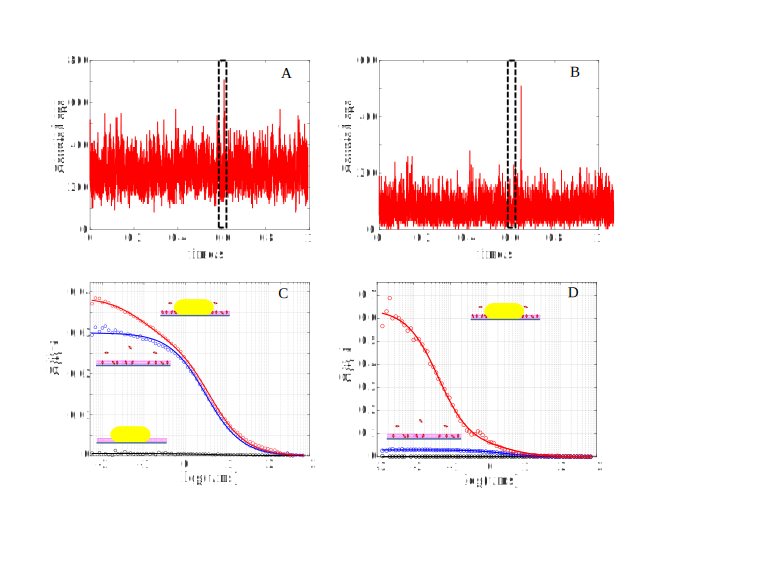
\includegraphics[width=0.8\textwidth]{corr_enhnc.png}
	\caption{Fluorescence correlation in high background. Fluorescence time trace of $100~$\nM ATTO 647N in the presence of a nanorod before (A) and after (B) lifetime filtering. The dashed boxes highlight a near-field burst in both traces. Autocorrelations of fluorescence intensity traces at $100~$\nM ATTO 647N before (C) and after (D) lifetime filtering. Red circles: correlation in presence of the rod; blue circles: correlation in the absence of the rod; black circles: correlation of the gold luminescence only (in absence of ATTO 647N).}
	\label{fig:corr_enhnc}
\end{figure}
The diffusion coefficient $4.44~\um^2/s$ obtained for ATTO 647N in the bilayer is close to the literature values of $3-4~\um^2/s$\cite{mach2010lipid} for other dyes and is similar to those of freely moving lipid molecules in the bilayer. No correlation component was observed for the dyes in the solution because of the low fluorescence intensity and high background from the dyes diffusing in the bilayer. In presence of a nanorod, we find the same long diffusion time again, corresponding to molecules diffusing in the diffraction-limited area, while we assign the shorter component to diffusion in the near-field of the gold nanorod, responsible for enhanced brightness of the molecules. The near-field width is about $10$ times smaller than the far-field diameter, and is consistent with near-field simulations and lifetime calculations around gold nanorods of this size.\cite{khatua2014resonant,seelig2007nanoparticleinduced} The near-field area is reduced by more than one order of magnitude ($70$ times in our case). Assuming the diffusion coefficient to be same in the far field and near field, and applying the analysis for a Gaussian near-field intensity distribution, we obtain a diffusion time of $57\pm11~\us$ in the near-field from the relation $\omega^2=4D\tau_N$. The peak ratio $5\pm1.5$ is close to the maximum enhancement factor of $4$ obtained from the burst analysis (vide supra) which confirms the results obtained in the FCS and shows that the maximum enhancement factor can simply be obtained from the FCS. However, the contrast of the near-field correlation ($0.01$) is much weaker, which may make it difficult to distinguish this component in FCS experiments with lower signal-to-noise ratios.\\

As can be seen in Fig.\ref{fig:corr_enhnc}A, C, the contrast of the near-field component is weak, essentially because it is reduced by background. To further enhance this correlation component, we can exploit a further difference between enhanced and unenhanced counts, namely their delay after excitation, less than $2~ns$ versus $3.7~ns$, respectively. We thus filtered out unenhanced photons by selecting photons detected within $1~ns$ from the excitation pulse, and computed their correlation function. A typical time trace before and after filtering can be seen in Fig. \ref{fig:corr_enhnc} A, B. The average background went down from $272~$kcps to $74~$kcps and the signal-to-noise ratio of the enhanced signal improves accordingly, as can be seen for the burst marked in the box. The contrast of the near-field component in the filtered correlation has now been enhanced by about $60$ times, making it easy to distinguish against the far-field correlation. From the filtered correlation in Fig.\ref{fig:corr_enhnc}D, we find a near-field diffusion time of $59\pm5~\us$, similar to the one deduced from the unfiltered correlation. Shorter filtering windows lead to even shorter times for this near-field component, corresponding to larger emission enhancement and quenching at shorter distances. However, this dependence is rather slow, so that the above number has physical meaning as the typical near-field diffusion time. Of course, filtering down to very short times considerably reduces the signal-to-noise ratio (See Fig. S\ref{SIfig:cutoff-effect})\\
\begin{figure}
	\centering
	\includegraphics[]{Zn_azurin_efcs.png}
	\caption{(A) Scheme showing the labeling strategy for protein anchoring onto the bilayer. The Azurin labeled with ATTO 655 and biotin binds to DSPE-PEG-Biotin in the bilayer through Neutravidin. (B) Autocorrelation of the time traces of the labeled protein in absence of the nanorod (blue), in the presence of the nanorod (red circles) and in the presence of the nanorod after lifetime filtering (solid red). Notice the higher correlation contrast after lifetime filtering in presence of nanorod.}
	\label{fig:Zn_azurin_efcs}
\end{figure}
The bilayer-nanorod platform can be used for biochemical applications. We demonstrate this by anchoring a protein, azurin, onto the bilayer. This protein with a copper metal center is known to mediate electron transfer in biological redox processes.\cite{kolczak2006azurin,Vijgenboom1997invivo} To prevent electron transfer processes in the present experiments, we used azurin with a zinc metal center. The protein's Lysine 122 residue was labeled with ATTO 655. As Zn-Azurin does not show electron transfer, electron transfer to or from the dye is excluded. The anchored protein shows free mobility on the bilayer as can be inferred from the single decay component of the autocorrelation (Fig.\ref{fig:Zn_azurin_efcs}B, blue). This component has a diffusion time of $22\pm5~ms$ in the far field, which is around five times longer than the diffusion time of the free dye ATTO 647N. We attribute this longer diffusion time to interactions and reduced mobility of the bulky anchoring among surrounding lipids. We now turn to the correlation curve in the presence of the nanorod. The absence of any long-lived correlation component indicates that the protein continues to diffuse freely and does not stick to the solid surfaces. The near-field diffusion time for the protein was found to be $318~\us$, which is also around five times the near field time of ATTO 647N. This confirms that diffusion is not significantly altered, even within $30~nm$ of the rod.\\
%===============================CONCLUSION==============================
\section{Conclusion}
A lipid bilayer substrate prevents the nonspecific sticking of dyes to a glass surface and thereby makes it possible to perform enhanced FCS around a metal structure with no hindrance in the diffusion kinetics. The fluorescence of molecules in the near field always decays faster than that of far-field molecules. The shorter lifetime of enhanced fluorescence can be used to discriminate the near-field signal from the high background in the far field. The autocorrelation of the shorter lifetime component shows spectacular improvement in the correlation contrast which is helpful for studying FCS at high concentrations in presence of a strong background from unenhanced molecules. The bilayer substrate with nanostructures can be used as a hybrid surface where probe molecules can either be functionalized to the surface or be kept free in the solution without any nonspecific interaction. As lipid bilayers are close to biological membranes, many kinds of biochemical FCS experiments on the bilayer at physiological concentrations can be envisioned.\\
\subsection{Supporting Information:}
Gold nanorod characterization, chemical structures, bilayer characterization, zoomed in intensity bursts, fitting model and calculations, lifetime-based selection, effect of lifetime selection, fluorescence enhancement in sucrose (3D) solution, partitioning of dye between bilayer and solution.
\subsection{Acknowledgement:}
We would like to thank Prof. Joerg Enderlein for his suggestion of using lifetime filtering for improving correlation contrast. This work was supported by the Netherlands Organization for Scientific Research (NWO/OCW), as part of the Frontiers of Nanoscience program.
% \bibliographystyle{achemso.bst}
\bibliography{efcs}
\end{document}